\documentclass[a4paper,oneside,14pt]{extreport}

\usepackage[T2A]{fontenc}
\usepackage[utf8]{inputenc}
\usepackage[english,russian]{babel}

%\usepackage[left=30mm, right=20mm, top=20mm, bottom=20mm]{geometry}
\usepackage[left=20mm, right=10mm, top=5mm, bottom=20mm]{geometry}

\usepackage{microtype}
\sloppy

\usepackage{setspace}
\onehalfspacing

\usepackage{indentfirst}
\setlength{\parindent}{12.5mm}

\usepackage{titlesec}
\titleformat{\chapter}{\LARGE\bfseries}{\thechapter}{14pt}{\LARGE\bfseries}
\titlespacing*{\chapter}{\parindent}{0mm}{5mm}
\titleformat{\section}{\Large\bfseries}{\thesection}{14pt}{\Large\bfseries}

\addto{\captionsrussian}{\renewcommand*{\contentsname}{Содержание}}
\usepackage{natbib}
\renewcommand{\bibsection}{\chapter*{Список использованных источников}}

\usepackage{caption}

\usepackage{wrapfig}
\usepackage{float}

\usepackage{graphicx}
\newcommand{\imgwc}[4]
{
	\begin{figure}[#1]
		\center{\includegraphics[width=#2]{inc/img/#3}}
		\caption{#4}
		\label{img:#3}
	\end{figure}
}
\newcommand{\imghc}[4]
{
	\begin{figure}[#1]
		\center{\includegraphics[height=#2]{inc/img/#3}}
		\caption{#4}
		\label{img:#3}
	\end{figure}
}
\newcommand{\imgsc}[4]
{
	\begin{figure}[#1]
		\center{\includegraphics[scale=#2]{inc/img/#3}}
		\caption{#4}
		\label{img:#3}
	\end{figure}
}

\usepackage{pgfplots}
\pgfplotsset{compat=newest}

\usepackage{listings}
\usepackage{listingsutf8}
\lstset{
	basicstyle=\footnotesize\ttfamily,
	keywordstyle=\color{blue},
	stringstyle=\color{red},
	commentstyle=\color{gray},
	numbers=left,
	numberstyle=\tiny,
	numbersep=5pt,
	frame=false,
	breaklines=true,
	breakatwhitespace=true,
	inputencoding=utf8/koi8-r
}

\lstdefinestyle{c}{
	language=C++,
	backgroundcolor=\color{white},
	basicstyle=\footnotesize\ttfamily,
	keywordstyle=\color{blue},
	stringstyle=\color{red},
	commentstyle=\color{gray},
	directivestyle=\color{orange},
	numbers=left,
	numberstyle=\tiny,
	stepnumber=1,
	numbersep=5pt,
	frame=single,
	tabsize=4,
	captionpos=t,
	breaklines=true,
	breakatwhitespace=true,
	escapeinside={\#*}{*)},
	morecomment=[l][\color{magenta}]{\#},
	columns=fullflexible
}

\newcommand{\code}[1]{\texttt{#1}}

\usepackage{amsmath}
\usepackage{amssymb}

\usepackage[unicode]{hyperref}
\hypersetup{hidelinks}

\makeatletter
\newcommand{\vhrulefill}[1]
{
	\leavevmode\leaders\hrule\@height#1\hfill \kern\z@
}
\makeatother

\begin{document}

\chapter*{Лабораторная работа 1}
Цель: изучение дискретного преобразования Фурье в Matlab.
\section*{Задание 1 – анализ сгенерированного сигнала}
Сгенерировать сигнал продолжительностью 90 лет с шагом месяц => всего будет $90*12=1080$ шагов. Сигнал содержит косинус периодом 1 год, синус периодом 8.86 года и еще один косинус периодом 18.6 года => период 1-ой функции $12$ месяцев, 2-ой $8.86*12=106.32$ месяцев и 3-ей функции $12*18.6=223.2$ месяцев. Начало - дата рождения (05.2000) => $2000*12+5=24005$ => начинаем с 24005-го месяца. Подбираем фазы так, чтобы нулевой аргумент годовой гармоники приходился на начало года,  8.86-летнего цикла – на начало 2024 года, 18.6-летнего цикла на начало 2006 года => $\phi_1=0, \phi_2=1.12*\pi, \phi_3=0.31*\pi$. Амплитуды сигналов выбрать в соответствии с правилом: 20+ номер по алфавиту первых букв Ваших ФИО => Пронин Арсений Сергеевич (ПАС - номера букв в алфавите = 16, 0, 18) $A_1=36, A_2=20, A_3=38$.

Выполнить спектральный анализ сигнала, построить график амплитудного спектра (рис. \ref{task1_ampl_spectr}):
\newline
\begin{figure}[h]
	\center{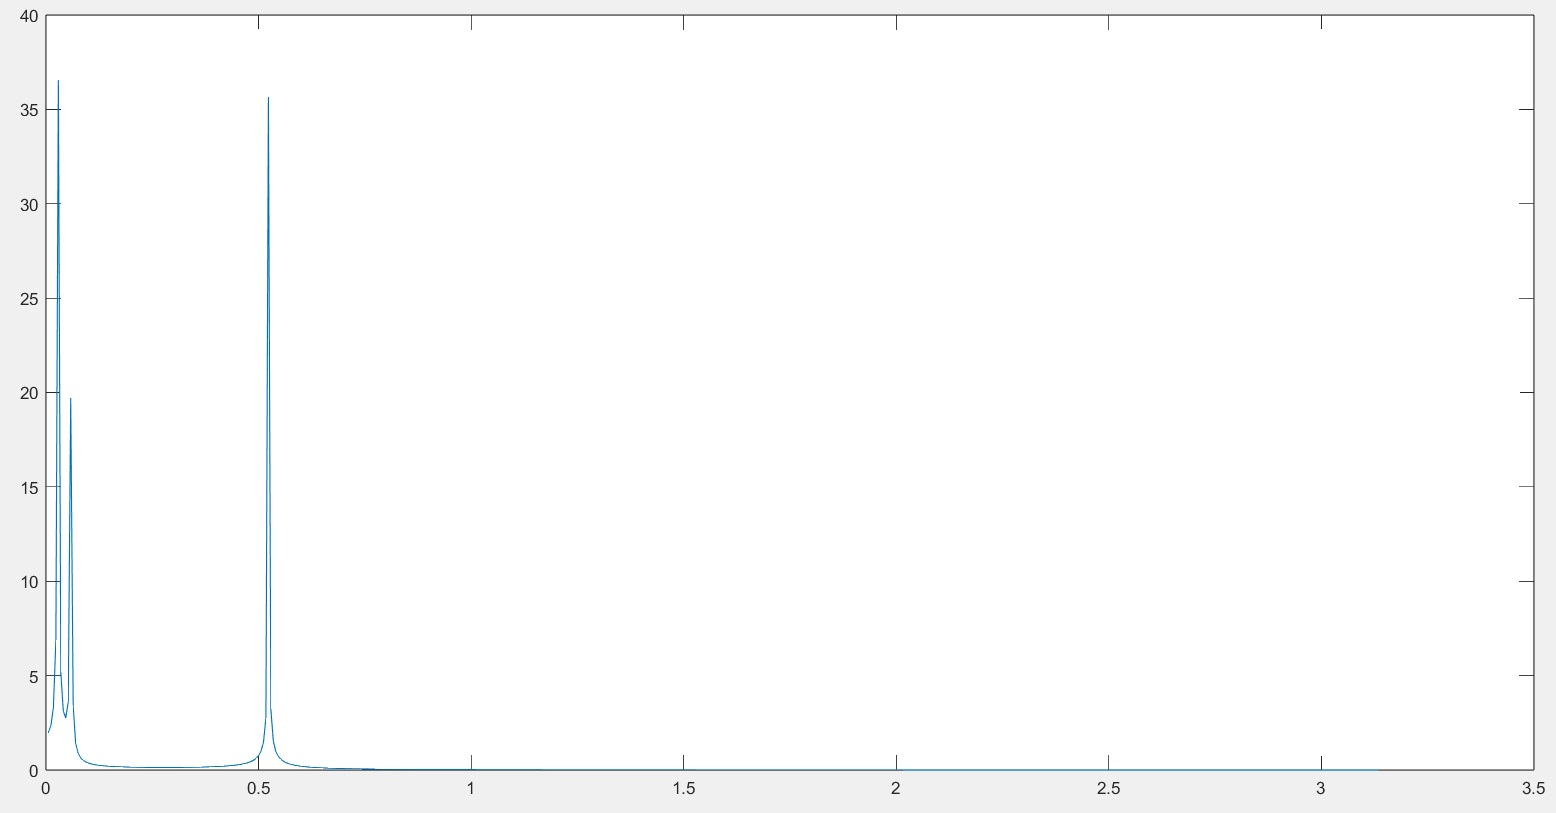
\includegraphics[width=1\linewidth]{inc/task1_ampl_spectr}}
	\caption{График амплитудного спектра}
	\label{task1_ampl_spectr}
\end{figure}

\begin{figure}[h]
	\center{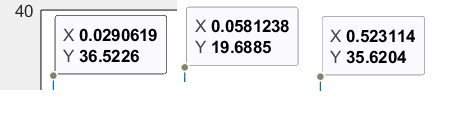
\includegraphics[width=1\linewidth]{inc/task1_ampl_spectr_vals}}
	\caption{Пиковые значения}
	\label{task1_ampl_spectr_vals}
\end{figure}

На рисунке \ref{task1_ampl_spectr_vals} видно что пиковые значения Y близки к амплитудам, а соответствующие им X $\approx$ циклическим частотам.

\section*{Задание 2 – фурье-анализ реального сигнала}
Считать из бюллетеня EOP C01 службы вращения Земли данные UT-TAI (6-я колонка) и построить график (рис. \ref{task2_g1}):

\begin{figure}[h]
	\center{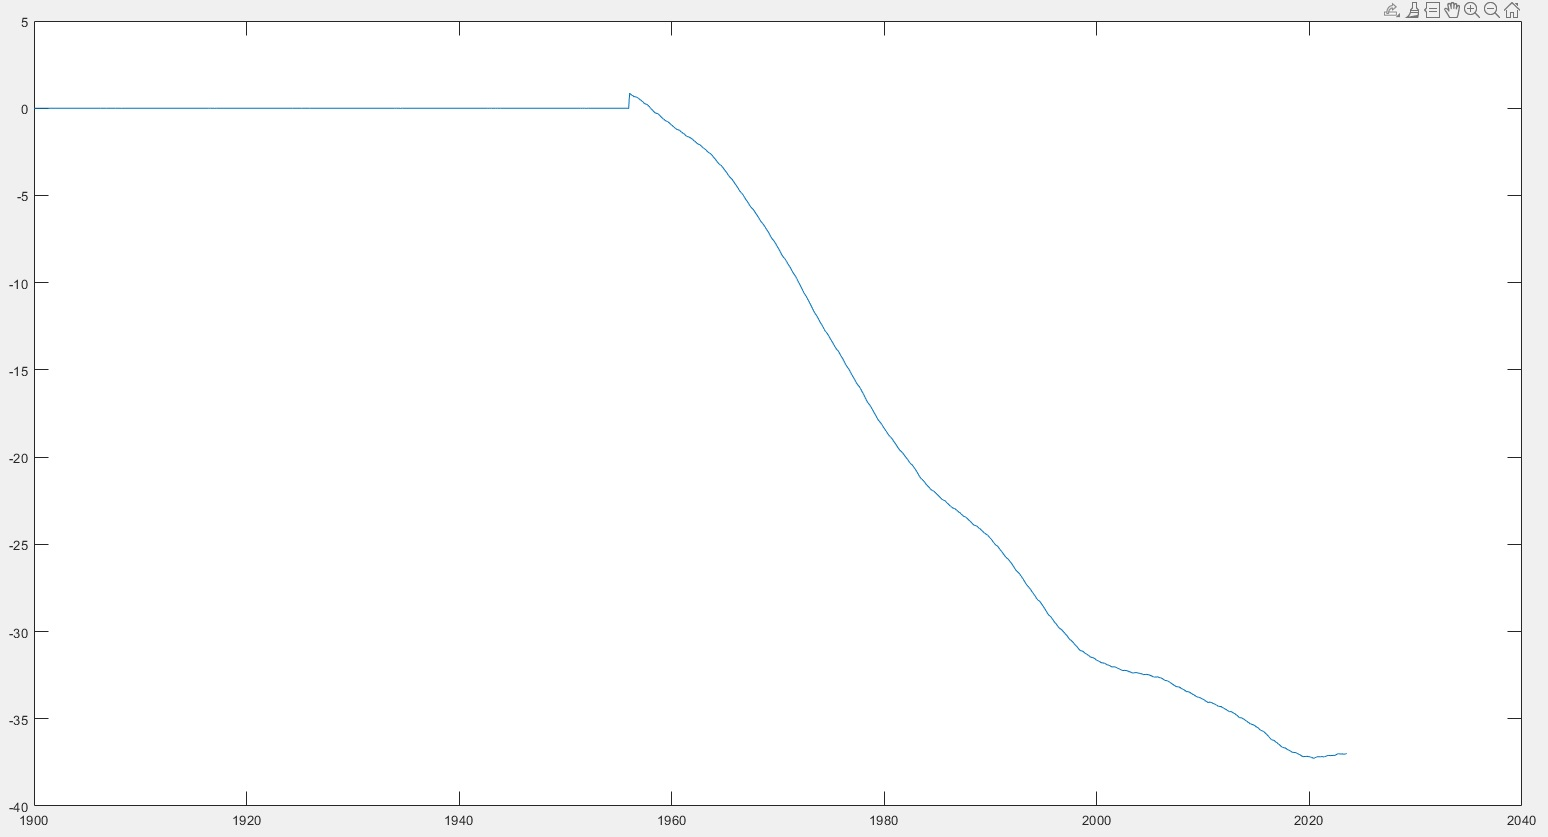
\includegraphics[width=1\linewidth]{inc/task2_g1}}
	\caption{Зависимость UTTAI от YEARS}
	\label{task2_g1}
\end{figure}

\newpage
Продифференцировать данные, получив LOD (минус производная, рис. \ref{task2_g2}):

\begin{figure}[h]
	\center{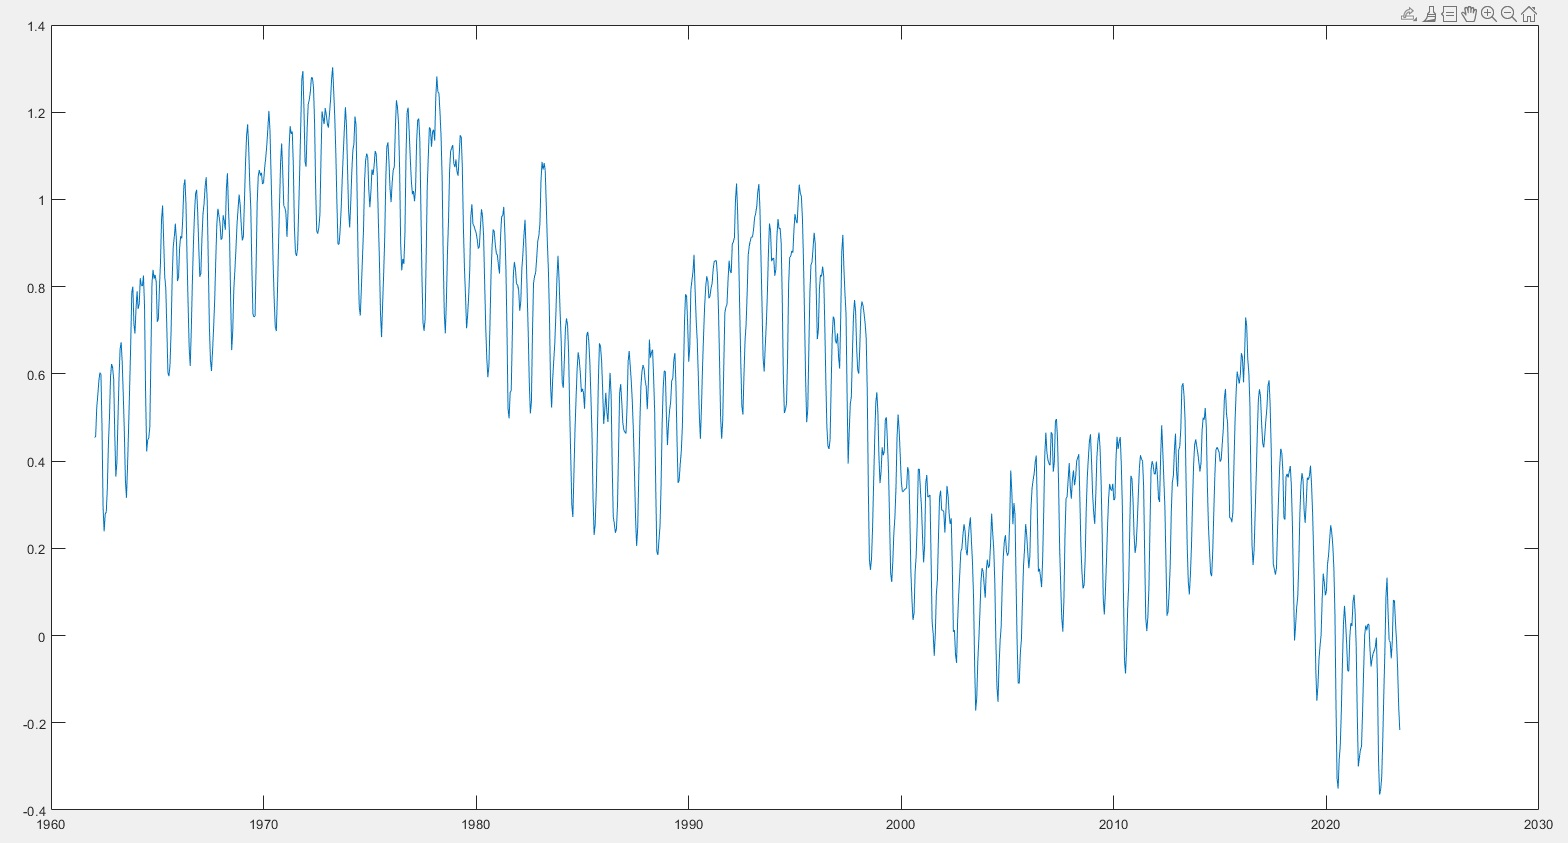
\includegraphics[width=0.93\linewidth]{inc/task2_g2}}
	\caption{Зависимость LOD от YEARS c 1962-го года}
	\label{task2_g2}
\end{figure}

Взять ряд с 1962 года  и вычислить его спектр. Построить график амплитудного спектра по частотам (рис. \ref{task2_g3}):

\begin{figure}[h]
	\center{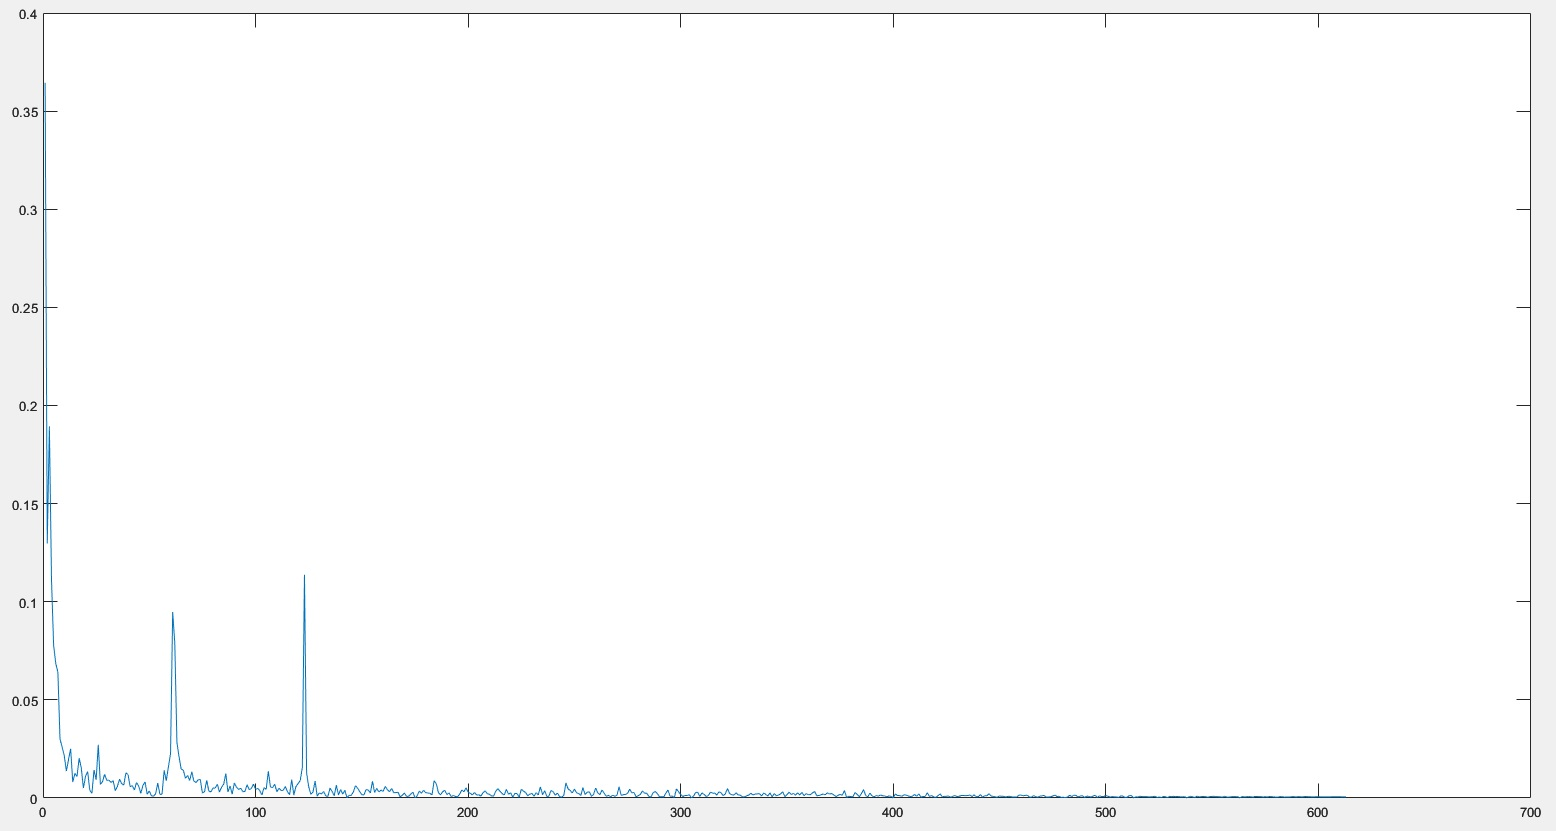
\includegraphics[width=0.93\linewidth]{inc/task2_g3}}
	\caption{График амплитудного спектра по частотам LOD c 1962-го года}
	\label{task2_g3}
\end{figure}

\newpage
По пиковым значениям (рис. \ref{task2_freq_vals}) можно определить циклические частоты: 

$0.00511244$

$0.311859$

$0.62883$

%и Периоды:
%
%$\Large \frac{2 \cdot \pi}{0.00511244} \approx 1229$ лет
%
%$\Large \frac{2 \cdot \pi}{0.311859} \approx 20$ лет
%
%$\Large \frac{2 \cdot \pi}{0.62883} \approx 10$ лет

\begin{figure}[h]
	\center{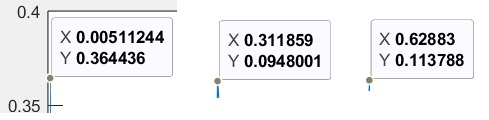
\includegraphics[width=1\linewidth]{inc/task2_freq_vals}}
	\caption{Значения частот}
	\label{task2_freq_vals}
\end{figure}

%\newpage
\section*{Задание 3 – построение спектра комплексного ряда}

Из того же файла считать вторую (x) и четвертую (y) колонки и объединить их в  комплексный временной ряд (x+iy). Построить график спектра как для положительных так и для отрицательных частот:

\begin{figure}[h]
	\center{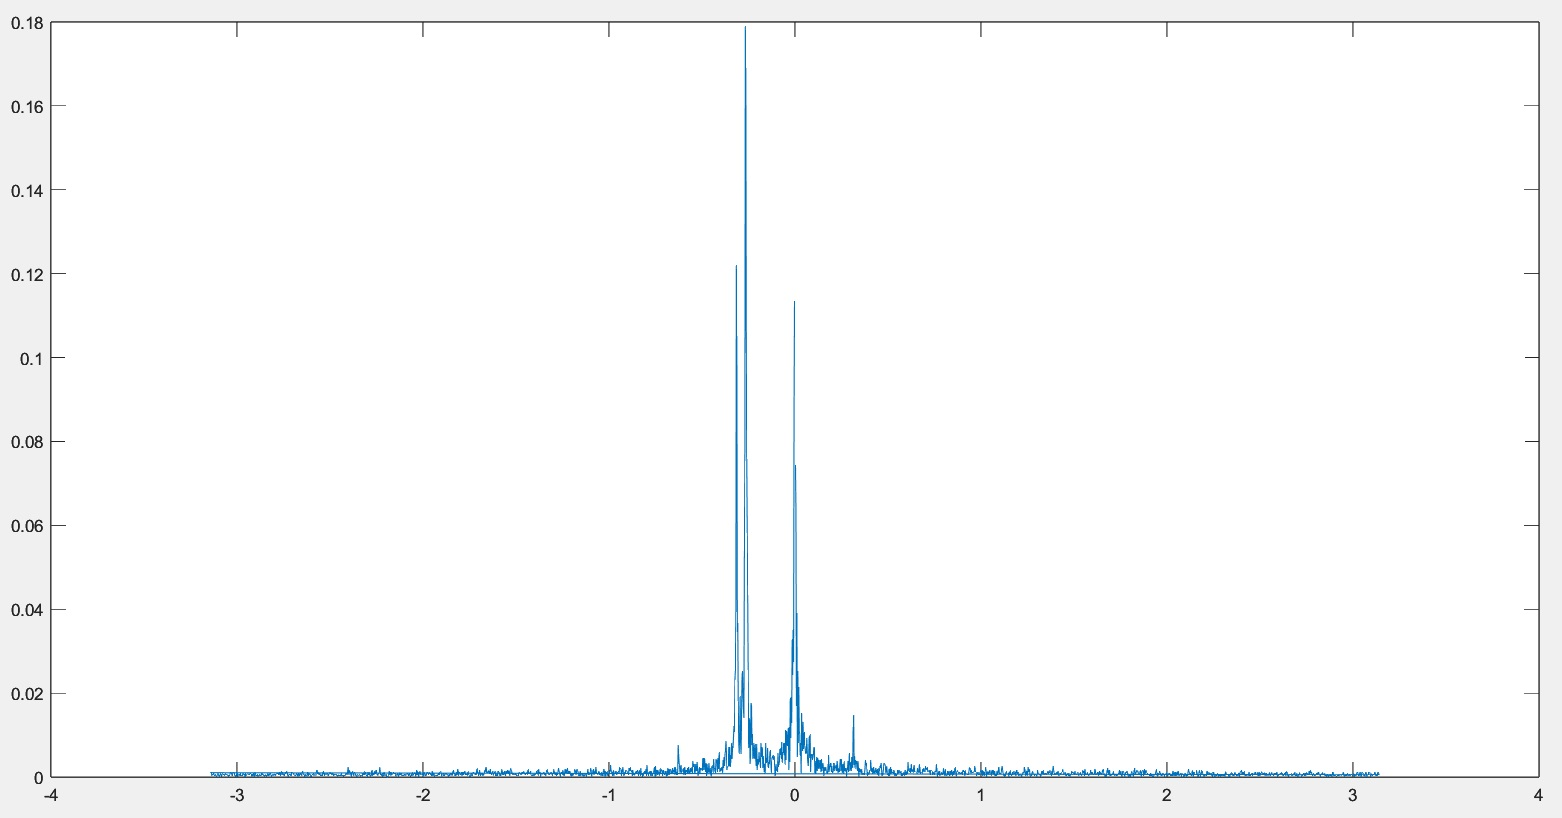
\includegraphics[width=1\linewidth]{inc/task3_g1}}
	\caption{График спектра}
	\label{task3_g1}
\end{figure}

\end{document}